% begin module related-rates-ex1
\begin{frame}
\begin{example} Water is poured into a conical container \alertNoH{ 6}{at the rate of 10
cm${}^3$/sec}.  The cone points directly down, and it has a height of
30 cm and a base radius of 10 cm.  \alertNoH{ 8}{How fast is the water level rising}
when the \alertNoH{ 8}{water is 4 cm deep}? \pause 
\begin{itemize}
\item To start, \textbf{draw a picture} and introduce variables/labels. \end{itemize} \pause 
\begin{columns}[c]
\column{.35\textwidth}
\hfill 
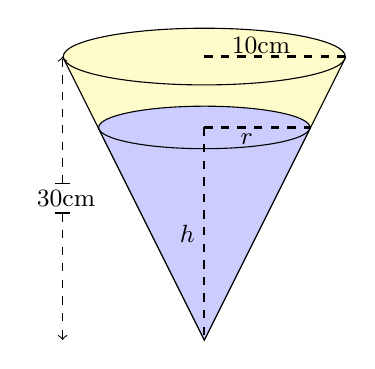
\begin{tikzpicture}[scale=.9]
        \draw [fill=yellow!20!white,opacity=1] (-1.99,3.98) -- (1.99,3.98) -- (0,0) -- cycle;
        \draw [fill=yellow!20!white,opacity=1,] (0,4) circle (1.99cm and 0.4cm);
        \draw [fill=blue!20!white,opacity=1] (-1.49,2.98) -- (1.49,2.98) -- (0,0) -- cycle;
        \draw [fill=blue!20!white,opacity=1] (0,3) circle (1.49cm and 0.3cm);
        \draw[dashed, thick] (0,4) -- (2,4);
        \draw[dashed, thick] (0,3) -- (1.5,3);
        \draw[dashed, thick] (0,3) -- (0,0);
        \draw[dashed, arrows=|->](-2,1.8)--(-2,0);
        \draw[dashed, arrows=|->](-2,2.2)--(-2,4);
        \node[above] at (0.8,3.9) {  \small  $10$cm};
                \node[below] at (0.6,3.05)  { \small  $r$};
                \node[left] at (0,1.5)  {  \small  $h$};
                \node[right] at (-2.5,2) { \small  $30$cm};
    \end{tikzpicture} 
\column{.65\textwidth}
  At time $= t $ seconds let\\
  $r=r(t)$  be the surface radius (cm) of the water,\\ 
  $ h=h(t) $ be the height (cm) of the water,\\
  $ V=V(t) $ be the volume of water in the tank.
 \pause 
\textbf{ Identify and given and required rates:}\\
\pause 
 Given:  \pause  \alertNoH{ 6}{ ${\frac{\diff V}{\diff t} = 10}$ cm$ {}^3 $/s} \pause \\
  Required: \pause Find \alertNoH{ 8}{ $ \frac{\diff h}{\diff t} $} when \alertNoH{ 8}{$ h=4.$} 
 
\end{columns}

\end{example}
\end{frame}

\begin{frame}
\begin{example}
\begin{columns}[c]
\column{.25\textwidth}
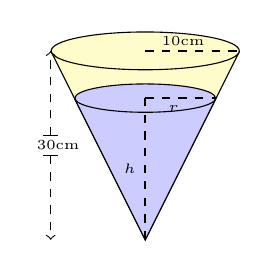
\begin{tikzpicture}[scale=.6]
        \draw [fill=yellow!20!white,opacity=1] (-1.99,3.98) -- (1.99,3.98) -- (0,0) -- cycle;
        \draw [fill=yellow!20!white,opacity=1,] (0,4) circle (1.99cm and 0.4cm);
        \draw [fill=blue!20!white,opacity=1] (-1.49,2.98) -- (1.49,2.98) -- (0,0) -- cycle;
        \draw [fill=blue!20!white,opacity=1] (0,3) circle (1.49cm and 0.3cm);
        \draw[dashed, thick] (0,4) -- (2,4);
        \draw[dashed, thick] (0,3) -- (1.5,3);
        \draw[dashed, thick] (0,3) -- (0,0);
        \draw[dashed, arrows=|->](-2,1.8)--(-2,0);
        \draw[dashed, arrows=|->](-2,2.2)--(-2,4);
        \node[above] at (0.8,3.9) {  \tiny  $10$cm};
                \node[below] at (0.6,3.05)  { \tiny  $r$};
                \node[left] at (0,1.5)  {  \tiny  $h$};
                \node[right] at (-2.5,2) { \tiny  $30$cm};
    \end{tikzpicture}
    
\onslide<4->{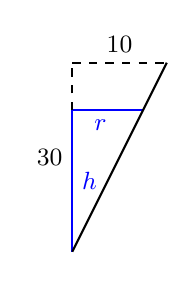
\begin{tikzpicture}[scale=.6]
        \draw[dashed,  thick] (0,4) -- (2,4);
        \draw[thick, color=blue] (0,3) -- (1.5,3);
        \draw[thick, color=blue] (0,3) -- (0,0);
        \draw[thick] (0,0) -- (2,4);
        \draw[dashed,thick] (0,3) -- (0,4);
         %\draw[dashed, arrows=<->](-2,4)--(-2,0);
         \node[above] at (1,4) {  \small  $10$};
        \node[below, color=blue ] at (0.6,3)  { \small  $r$};
        \node[right,color=blue ] at (0,1.5)  {  \small  $h$};
        \node[left] at (0,2) { \small  $30$};
    \end{tikzpicture}    
}    
\column{.65\textwidth}
 
 Given:      $\displaystyle {\frac{\diff V}{\diff t} = 10}$ cm/s,  Find: $ \displaystyle \frac{\diff h}{\diff t} $ when $ h=4.$ 

\textbf{Find an equation  relating quantities whose rates are given or required:}\\ \pause
\[
V=\frac13\pi r^2h
\]
\pause We do not have the rate of $ r $ either given or required, so we eliminate it from this equation.  \pause 
 Similar triangles (or equivalently, by taking $ \tan $ of the bottom angle) gives $ \displaystyle \frac{r}{h}=\frac{10}{30} $, so $ \displaystyle r = \frac{1}{3}h $.\\ \pause 
\end{columns}

This gives us 
\[
V=\frac13\pi r^2 h=\frac13 \pi \left(\frac{h}{3}\right)^2 \cdot h =\frac{1}{27}\pi h^3
\] 

\end{example}
\end{frame}


\begin{frame}
\begin{example}
\[
V= \frac{\pi}{27} h^3
\] 

\textbf{Differentiate} (implicitly with respect to $ t $):\\
\[
 \frac{\diff V}{\diff t}=\frac{\pi}{9}  h^2 \cdot h'(t)
\]
\pause 
We are interested in \textbf{evaluating} $ h'(t) $ when  $h=4$cm and $V'(t) =
10$ cm$ ^3 $/s.  \pause 
Putting this information into our last equation gives:
\[
h'(t)= \frac{9}{\pi h^2}\cdot V'(t)= \frac{9}{\pi\cdot 4^2}\cdot 10= \frac{90}{16\pi}\text{ cm/s} 
\]
thus $s'(t)=400$ km/h.

\end{example}
\end{frame}

% end module related-rates-ex1
